\label{sec:evaluation}

We conducted a pilot study of VizAPI on an 85-project subset of the
Duets benchmarks~\cite{durieux21}. Our study included 10 libraries and
their clients. For libraries, we pick the most popular Maven repositories 
in different categories such as logging and json parsing. We pick clients partly
from popular Github repositories and partly from Duets~\cite{durieux21}.
We collect both static and dynamic data for these projects.

\begin{figure*}[h]
\begin{center}
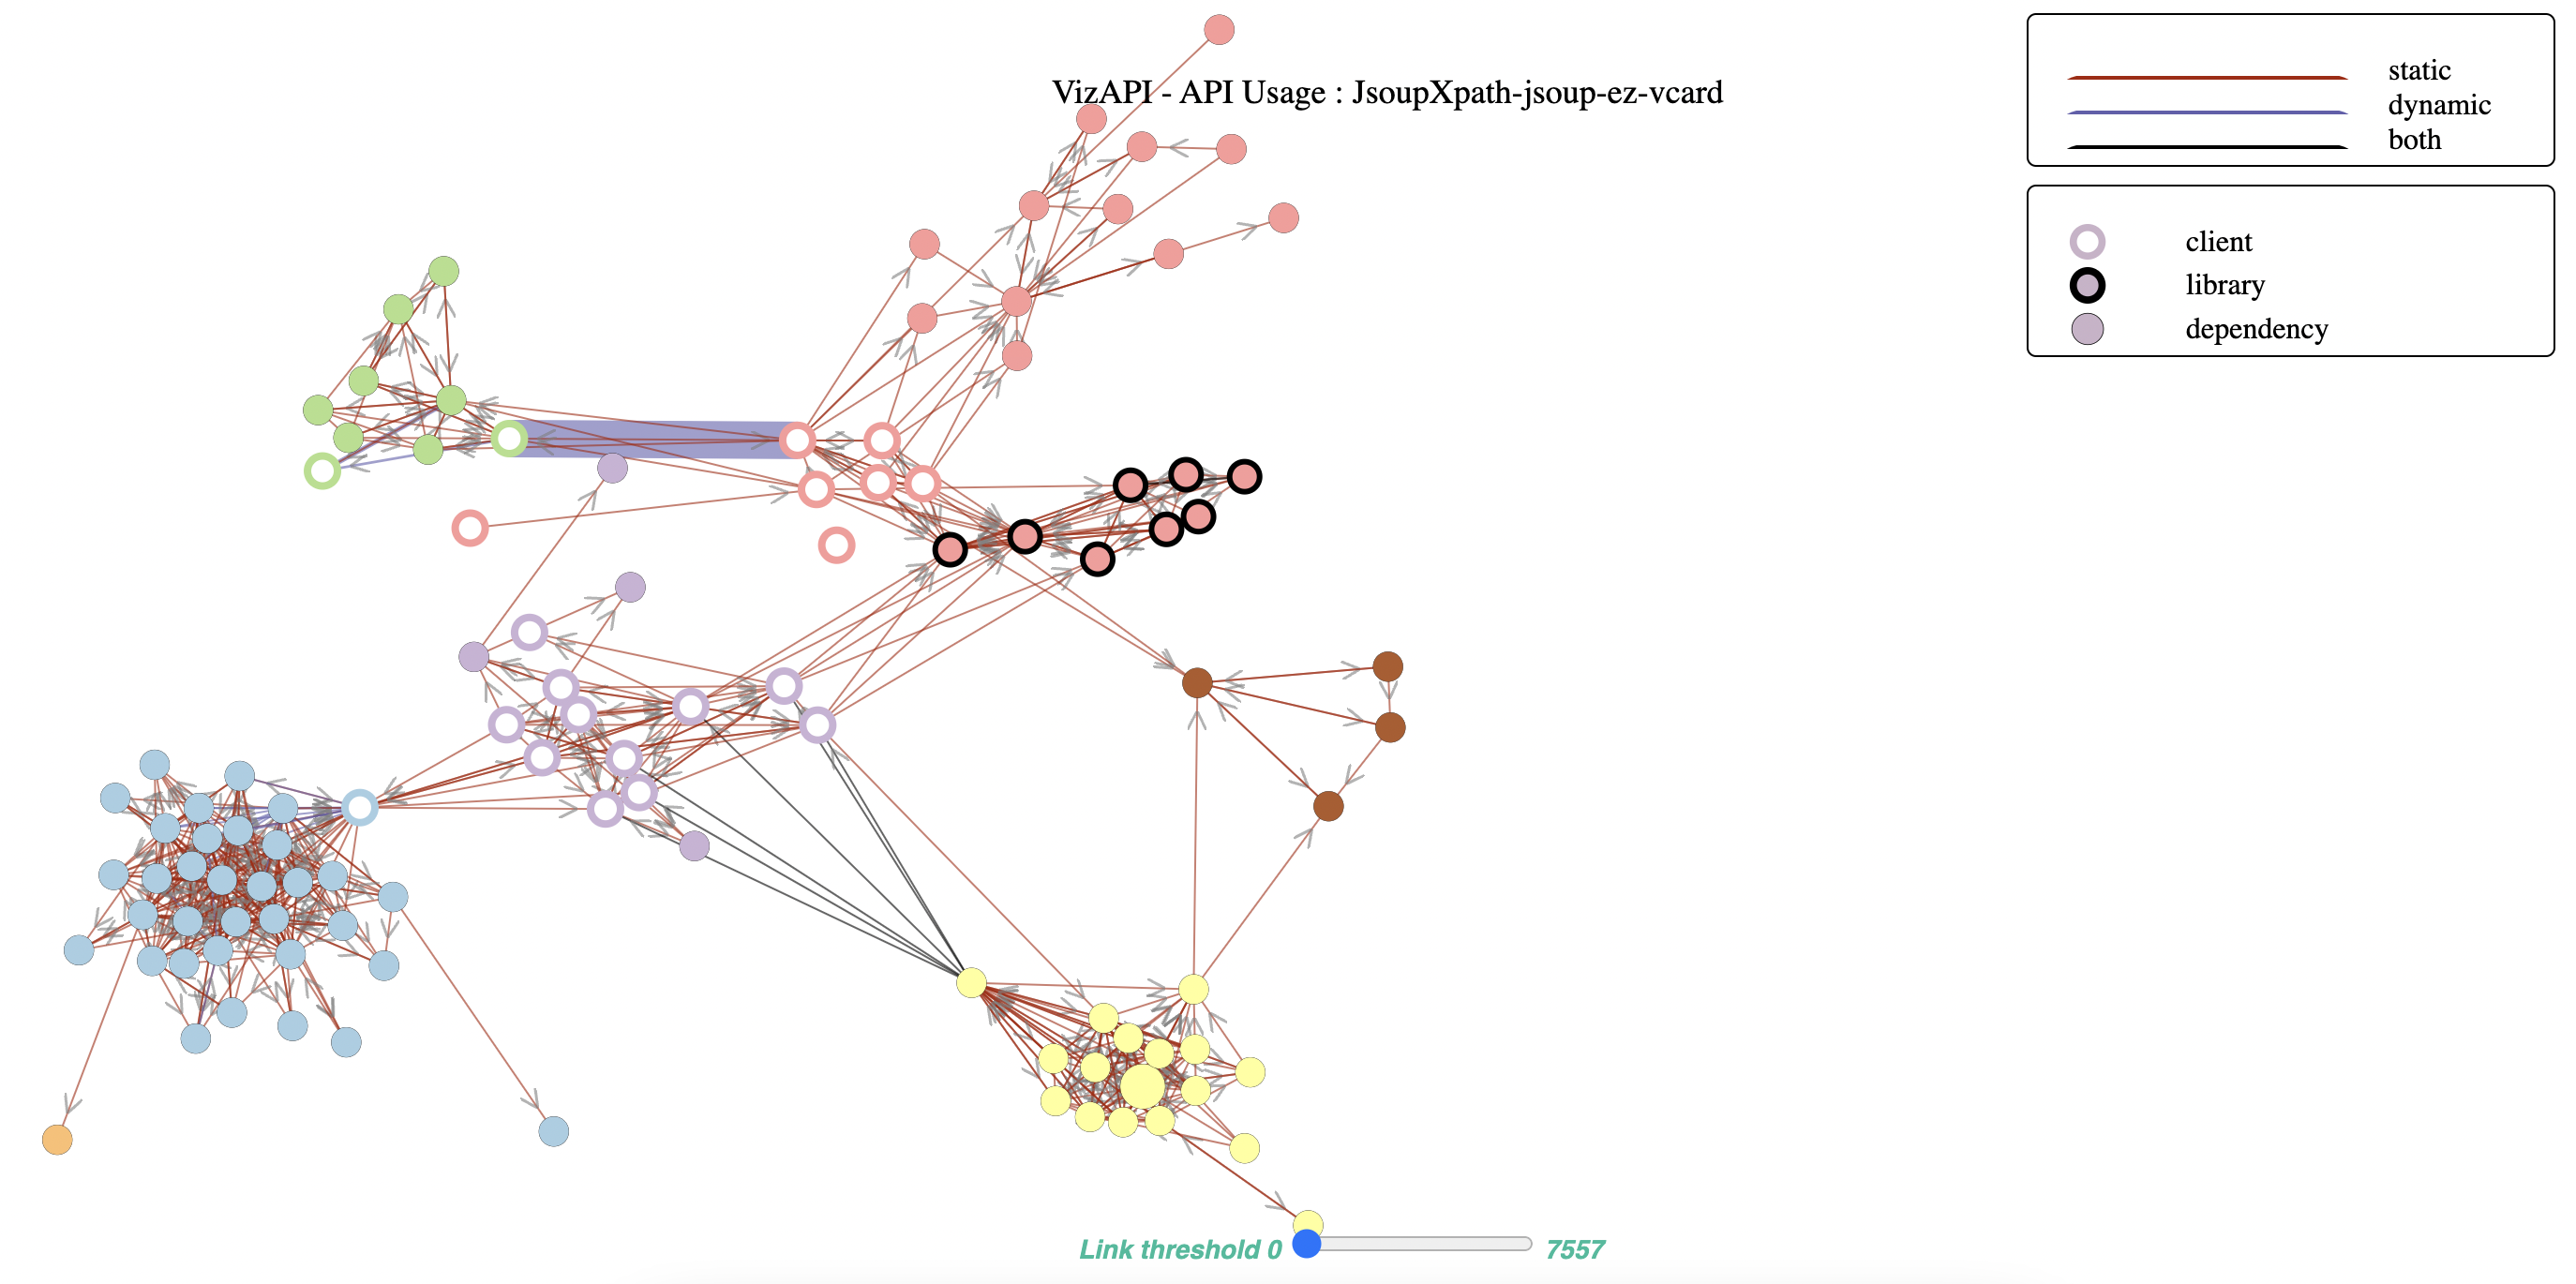
\includegraphics[scale=1,width=18cm,height=8cm]{images/usage-scenario1.png}
\caption{Usage Scenario 1: jsoup (library), JsoupXpath (client), ez-vcard (client)}
\label{fig:usagescenario1}
\end{center}
\end{figure*}

Now, we walk through an example usage scenario of VizAPI.
The graph in Figure~\ref{fig:usagescenario1} represents static and dynamic interactions of 2 clients with the jsoup\footnote{\url{https://github.com/jhy/jsoup}\label{jsoup}} library. Our clients are JsoupXpath\footnote{\url{https://github.com/zhegexiaohuozi/JsoupXpath}\label{jsoupxpath}} and ez-vcard\footnote{\url{https://github.com/mangstadt/ez-vcard}\label{ez-vcard}}.

We can start our exploration with the cluster of pink nodes. Many of these nodes belong to either JsoupXpath or jsoup. When we hover over them, the hover hints tell us that the client JsoupXpath calls directly into \texttt{org.jsoup.nodes} and \texttt{org.jsoup.select}. Notably, and as we might expect, we can see that \texttt{org.jsoup.helper} and \texttt{org.jsoup.internal} aren't called directly by JsoupXpath. This would mean that breaking changes in \texttt{org.jsoup.helper} or \texttt{org.jsoup.internal} wouldn't directly affect JsoupXpath\footnote{As a specific example, the retraction of an internal jsoup API would not break this client. Behavioural changes that are directly passed through to the external API, e.g. through delegation, can still break clients, but we can consider those to be changes in the external API.} Similarly, ez-vcard directly calls into \texttt{org.jsoup}.

ez-vcard also calls into jackson-core\footnote{\url{https://github.com/FasterXML/jackson-core}\label{jackson-core}} and jackson-databind\footnote{\url{https://github.com/FasterXML/jackson-databind}\label{jackson-databind}}, which are very tightly coupled amongst their own packages and with each other. This could mean that breaking changes in these libraries can propagate to many of their own packages.
.

